\section{Two-Moment Model}
\label{se:Two-MomentModel}

\subsection{Transport Equations}
Consider neutrino transport through static dense matter with only emission, absorption and isotropic iso-energetic scattering.
The Boltzmann equation after scaling to dimensionless units ($k_{B} = c = 1$) can be written as
\begin{equation}
  \pd{f}{t}+\vect{\ell}\cdot\nabla f
  =\f{1}{\tau}\,\cC(f).
  \label{eq:boltzmann}
\end{equation}
The distribution function $f = f(\omega,\varepsilon,\vect{x},t)$ gives the number of neutrinos propagating in the direction $\omega\in\bbS^{2}$, with energy $\varepsilon\in\bbR^{+}$, at position $\vect{x}\in\bbR^{3}$ and time $t\in\bbR^{+}$.  
$\vect{\ell} = \vect{\ell}(\omega)\in\bbR^{3}$ is the unit vector parallel to the neutrino three-momentum direction: $\vect{p}=\varepsilon\,\vect{\ell}$.
On the right-hand side, $\tau$ is collision time scale: $\tau\ll1$ for opaque regions where neutrinos have frequent interactions with the background; $\tau\gg1$ for transparent regions where neutrinos rarely interact with the background and stream freely.
$\cC(f)$ is the collision term, which models emission, absorption, and isotropic and elastic scattering: 
\begin{equation}
  \cC(f)=\xi\,\big(\,f_{0}-f\,\big)
  +(1-\xi)\,\big(\,\f{1}{4\pi}\int_{\bbS^{2}}f\,d\omega-f\,\big),
  \label{eq:collisionTerm}
\end{equation}
with $\xi = \sigma_{\Ab} / (\sigma_{\Ab}  + \sigma_{\Scatt} )$: $\xi = 1$ when the scattering opacity $\sigma_{\Scatt} = 0$ corresponding to pure emission and absorption; $\xi = 0$ when the absorption opacity $\sigma_{\Ab} = 0$ corresponding to pure scattering. 
$f_{0}$ is the neutrino equilibrium distribution function, which has the following form:
\begin{equation}
  f_{0}(\vect{z})=\f{1}{e^{(\varepsilon-\mu(\vect{x}))/T(\vect{x})}+1}.
  \label{eq:fermiDirac}
\end{equation}
$T(\vect{x})$ is the temperature in energy units and $\mu(\vect{x})$ is the neutrino chemical potential.
Both of them depend on the properties of the background as a function of $\vect{x}$.

\subsection{Two-Moment Model}
An approximate solution of the Boltzmann equation, Eq.~\eqref{eq:boltzmann}, can be found by employing a two-moment model.
Define the angular moments of the distribution function as follows
\begin{equation}
  \big\{\,\cJ,\vect{\cH},\vect{\cK}\,\big\}(\vect{z},t)
  =\f{1}{4\pi}\int_{\bbS^{2}}f(\omega,\vect{z},t)\,\{\,1,\vect{\ell},\vect{\ell}\otimes\vect{\ell}\,\}\,d\omega,
  \label{eq:angularMoments}
\end{equation}
where $\vect{z}:=\{\varepsilon,\vect{x}\}$.
The zeroth moment, $\cJ$, is referred to as the particle density.
The first moment, $\bcH$, is the particle flux, and the second moment, $\bcK$, is the stress tensor.
We can integrate Eq.~\eqref{eq:boltzmann} to obtain equations for the zeroth and the first moments
\begin{equation}
  \pd{\vect{\cM}}{t}+\nabla\cdot\vect{\cF}=\f{1}{\tau}\,\vect{\cC}(\vect{\cM}),
  \label{eq:momentEquations}
\end{equation}
with $\vect{\cM}=(\cJ,\vect{\cH})^{T}$, $\vect{\cF}=(\vect{\cH},\vect{\cK})^{T}$, and
\begin{equation}
  \vect{\cC}(\vect{\cM})=\vect{\eta}-\vect{\cD}\,\vect{\cM},
  \label{eq:collisionTermMoments}
\end{equation}
where $\vect{\eta}=(\xi\,f_{0},\vect{0})^{T}$, $\vect{\cD}=\mbox{diag}(\xi,\vect{I})$, and
$\vect{I}$ is the identity matrix.
Therefore, solving the Boltzmann equation, Eq.~\eqref{eq:boltzmann}, for the neutrino distribution function, $f(\omega,\vect{z},t)$, is approximated by solving the two-moment equations for the neutrino number density, $\cJ(\vect{z},t)$, and flux, $\bcH(\vect{z},t)$.

\subsection{Algebraic Closures }
As is shown in the previous section, the moment equation for $\bcH$ involves $\bcK$ and the two-moment system is open. 
To close the two-moment system, an algebraic closure is constructed.
For a two-moment method, algebraic closures give an approximate $\bcK$ based on the lower moments as follows:
\begin{equation}
\bcK = \vect{k} \cJ,
\end{equation}
where $\vect{k}$ is the Eddington tensor.
For example, assuming the neutrino distribution is symmetric about a preferred direction $\widehat{\vect{h}}=\vect{\cH}/|\vect{\cH}|$, Levermore\cite{levermore_1984} proposed
\begin{equation}
  \vect{k}=\f{1}{2}\big[\,\big(1-\chi\big)\,\vect{I}+\big(3\,\chi-1\big)\,\widehat{\vect{h}}\otimes\widehat{\vect{h}}\,\big],
  \label{eq:eddingtonTensor}
\end{equation}
where $\chi=\chi(\cJ,|\vect{\cH}|)$ is the Eddington factor. 

\subsection{Constraints on the Moments}
Neutrinos are fermions, and obey the Pauli exclusion principle, i.e. $f \in [0,1]$.
As a result, the angular moments of $f$ and the Eddington factor $\chi$ are constrained as follows\cite{levermore_1984,lareckiBanach_2011,kershaw_1976,shohatTamarkin_1943}: 
\begin{align}
\cJ \in[0,1], \quad &(1-\cJ)\cJ-|\vect{\cH}| \geq 0, \label{eq:MomentsBounds}\\
  \chi_{\mbox{\tiny min}}
  =\max\big(1-\f{2}{3\cJ},h^{2}\big)
  \leq & \chi \leq \min\big(1,\f{1}{3\cJ}-\f{\cJ}{1-\cJ}h^{2}\big)=\chi_{\mbox{\tiny max}},
  \label{eq:eddingtonFactorBounds}
\end{align}
where $h = |\bcH|/\cJ$ is the flux factor.

The constraints in Eq.~\eqref{eq:MomentsBounds} define realizable $\bcM$, which define a convex set in the $\cJ$-$\bcH$ space.
As we will see later in Section \ref{se:SpacialDiscretization}, this convexity makes a constraint-preserving spatial discretization possible.

The inequalities in Eq.~\eqref{eq:eddingtonFactorBounds} deserve more attention than has been given.
They have equal importance relative to the inequalities in Eq.~\eqref{eq:MomentsBounds} in maintain consistency with respect to Fermi-Dirac statistics.
The Eddington factor given by the algebraic closures discussed in \cite{murchikova_etal_2017} are examined in this paper as examples.
We consider various occupancies and plot $\cJ = 0.1$ and $\cJ = 0.9$ as examples for low and high occupancy, respectively, in Fig.~\eqref{fig:EddingtonFactorsWithDifferentClosure}.
As the figure shows, not all algebraic closures satisfy the Eddington factor bounds, Eq.~\eqref{eq:eddingtonFactorBounds}: Kershaw\cite{kershaw_1976}, Wilson\cite{wilson_1975,leblancWilson_1970}, Levermore\cite{levermore_1984}, Minerbo \cite{minerbo_1978}, Janka 2\cite{janka_1992} may work fine in the neutrino low occupancy limit, but not for high occupancies; Janka 1\cite{janka_1991} can be in error in both cases.
The only algebraic closure that remains within the Eddington factor bounds among those plotted is Cernohorsky and Bludman's \cite{cernohorskyBludman_1994}.
Though Levermore closure and Minerbo closure don't conserve the bounds in the high occupancy limit, they are widely used: {O'Connor} and {Couch}\cite{oConnorCouch_2018}, Pan et al\cite{pan_etal_2018}, Glas et al\cite{glas_etal_2018}, and Just et al\cite{just_etal_2018} use Minerbo closure, and Vartanyan et al\cite{vartanyan_etal_2018}, Cabezon et al\cite{cabezon_etal_2018}, and Kuroda et al\cite{kuroda_etal_2016} use Levermore clsoure.
\rc{Add more discussion.}

\begin{figure}[h]
  \centering
  \begin{tabular}{cc}
    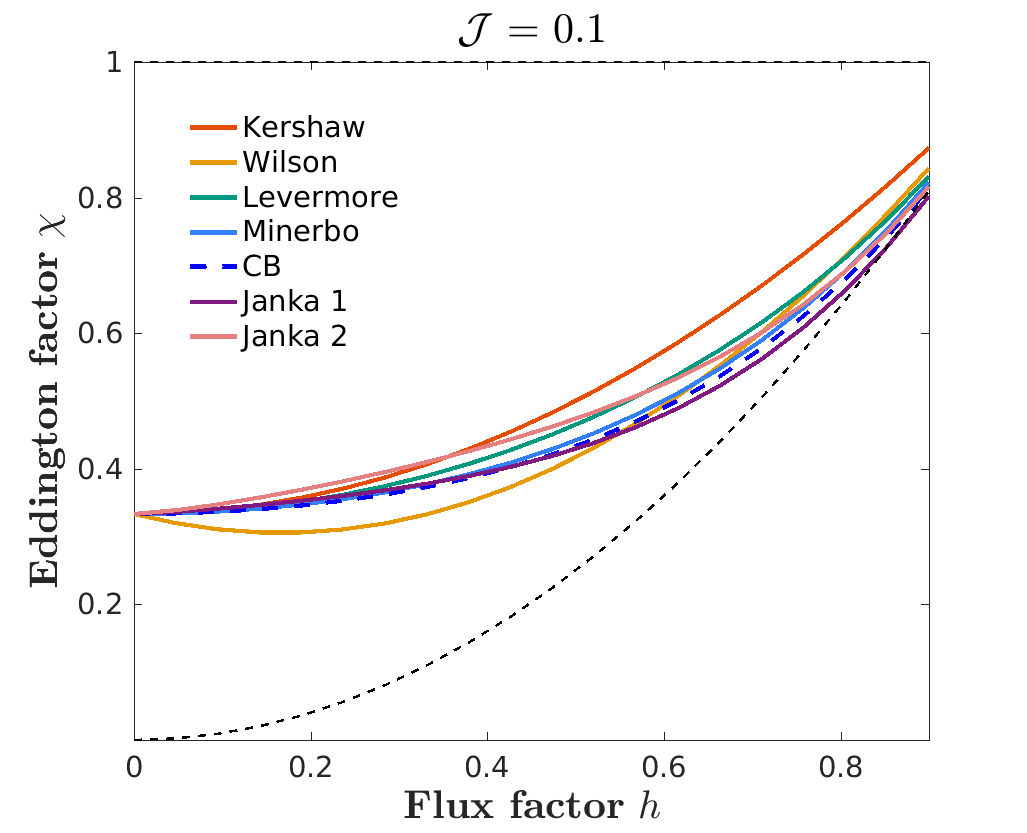
\includegraphics[width=0.5\textwidth]{figures/Closures0_10}
    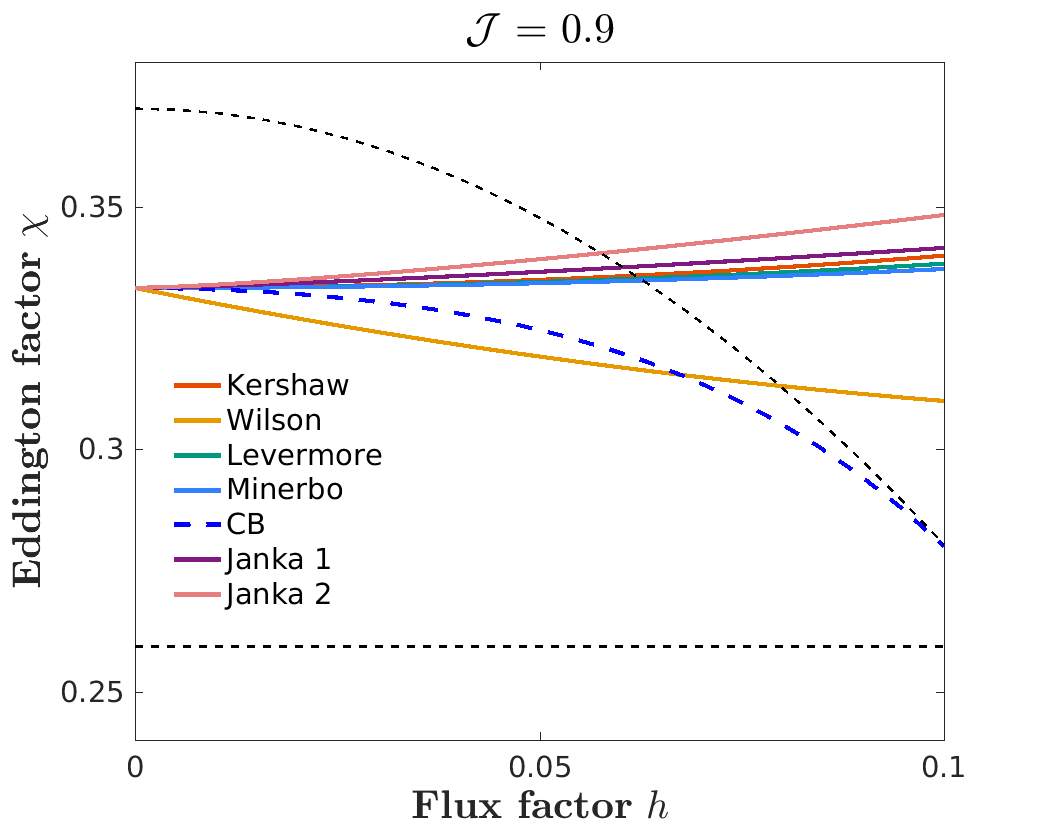
\includegraphics[width=0.5\textwidth]{figures/Closures0_90}
  \end{tabular}
   \caption{Plot of Eddington factors $\chi$ versus flux factor $h$ for different values of $\cJ$ for various algebraic closures: $\cJ=0.1$ (left panel, low occupancy) and $\cJ=0.9$ (right panel, high occupancy).  In each panel we plot the Eddington factors of Kershaw (red), Wilson (yellow), Levermore (green), Minerbo (light blue), Cernohorsky \& Bludman (blue) and Janka (purple and pink) closures.  We also plot $\chi_{\mbox{\tiny min}}$ and $\chi_{\mbox{\tiny max}}$, defined in Eq.~\eqref{eq:eddingtonFactorBounds} (lower and upper dashed black lines, respectively).}
  \label{fig:EddingtonFactorsWithDifferentClosure}
\end{figure}

